\documentclass{article}
\usepackage[utf8]{inputenc}
\usepackage{graphicx}
\graphicspath{{Images/}}

\title{CS 431 HW 1}
\author{Ethan Reinhart }
\date{October 2024}

\usepackage{multicol}
\usepackage{blindtext}
\usepackage{amsfonts}
\usepackage{caption}
\usepackage{listings}
\usepackage{xcolor}
\usepackage{graphicx}

\lstset{
    language=C,                    % Set language to C for syntax highlighting
    basicstyle=\ttfamily\footnotesize,  % Use smaller font size (footnotesize)
    keywordstyle=\color{blue},     % Keywords in blue
    commentstyle=\color{gray},     % Comments in gray
    stringstyle=\color{green},     % Strings in green
    showstringspaces=false,        % Don't show spaces in strings
    numbers=left,                  % Line numbers on the left
    numberstyle=\tiny\color{gray}, % Small gray line numbers
    stepnumber=1,                  % Line numbers at each line
    tabsize=4,                     % Tab size of 4 spaces
    breaklines=true,               % Break long lines
    breakatwhitespace=true,        % Only break at whitespace
    frame=single,                  % Frame the code
    keepspaces=true,               % Keeps spaces in text
    float=t,                       % Allows the listing to float like a figure
}

\begin{document}

\maketitle

\begin{multicols}{2}
\section{Introduction}
The irrational number $\pi$ is difficult to calculate to increasing precision. Most ways of calculating this number follow an algorithmic approach. Two such ways are the Riemann sum method and the Monte Carlo method.
The Riemann sum method revolves around a set number of slices, $n$, of the graph $x^2 + y^2 = 1$ for $y \geq 0$, where the area is found under this curve by multiplying $f(x) * 1/n$. The Monte Carlo method revolves around generating random numbers $a, b \in \mathbb{R}$ such that $a, b \in [-1, 1]$. The point $(a, b)$ is then checked to determine if it falls in the circle formed by $x^2 + y^2 = 1$. It should be obvious that both of these algorithms increase in precision with the number of slices or iterations used, respectively. The purpose of this paper is to use these algorithms as a benchmark to determine accuracy and speed when parallelizing these algorithms. A serial implementation of the Riemann sum approach is used as a benchmark while parallelized versions are used to compare the trade-offs between thread counts, different types of variables, and the number of steps (slices/iterations). We examine the difference between atomic and critical variables. We provide explanations as to why one is faster than the other. We examine varying the number of threads and provide logical reasoning behind speedups. Lastly, we examine different numbers of steps to validate performance with higher data thresholds.




\section{Atomic vs Critical}
Atomic and critical are both directives. Atomic allows access of a specific chunk of memory atomically, ensuring that race conditions are avoided by controlling thread access. Critical identifies a section of code that must be executed by a single thread at a time. The major difference between these two is that critical sets aside more memory and allocates more resources to create a critical section while atomic works over a single variable. By this, we would assume that atomic variables would outperform critical sections. Is this the case?
We examine atomic and critical variables, both directives over a single variable that is updated at the end of a threads' for loop. Here is the exact code (with critical used in this example):
\begin{lstlisting}
    #pragma omp parallel
    {
        double local_sum = 0.0;
        #pragma omp for
        for (int i = 0; i < num_steps; i++) {
                double x = i * step;
                double y = sqrt(1.0 - x * x) * step;
                local_sum += y;
        }
        #pragma omp critical
        sum += local_sum;
    }
\end{lstlisting}
As we can see, there is minimal overhead so we may expect these two to perform similarly. We are only accessing a shared variable once during a threads' lifecycle and this access is only to a single spot in shared memory. We first set the number of steps to be constant at 100,000,000 slices or iterations. We vary the thread count over $[7, 14, 21, 28]$. We set 28 to be the max as the Talapas architecture supports this. Each node on the server has 28 CPUs, each capable of processing a single thread concurrently. The results from executing the Riemann sum estimation in parallel are shown below:

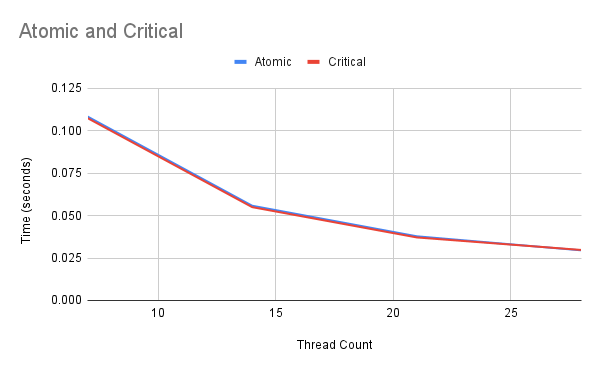
\includegraphics[width=\linewidth]{Images/actc.png}
\captionof{figure}{Atomic vs Critical : 100,000,000 steps with Varying Thread Count}

As we can see they perform almost analogously. We know further that varying the number of steps wouldn't provide significant insight to variance as large step sizes would not affect thread counts and each thread accesses shared memory only once in its lifecycle. We see that they perform roughly analogously likely due to their structure. Atomic variables declare sum to be a local variable accessed atomically where critical sections defined where a process executes. Both handle race conditions. For the provided code, they function practically identically leading to a statistically insignificant difference between how the two would vary. This lets us conclude that they are relatively interchangeable when working with a specific variable in shared memory. We cannot conclude anything about working with a large critical section from this.

\section{Serial vs Riemann Sum vs Monte Carlo}
The three methods are the only used throughout the project and are described in detail in the Introduction. We use serialized as the baseline for testing without parallelism. Here, we compare accuracy and speed for the Riemann Sum vs Monte Carlo. Here is the code for the Rieman Sum (the parallelized is the same but with OMP directives):
\begin{lstlisting}
    double calcPi_Serial(int num_steps)
    {
        double sum = 0.0;
        double step = 1.0 / num_steps;
    
        for (int i = 0; i < num_steps; i++) {
            double x = i * step;
            sum += sqrt(1.0 - x * x) * step;
        }
    
        return sum * 4;
    }
\end{lstlisting}
This code calculates the area under the curve $x^2 + y^2 = 1$ in the first quadrant and then multiplies by 4.
Here is the code for the Monte Carlo simulation.
\begin{lstlisting}
    double calcPi_P2(int num_steps)
    {
        int in_circle = 0;
    
        #pragma omp parallel
        {
                uint32_t my_seed = omp_get_thread_num();
                int temp_in_circle = 0;
                #pragma omp for
                for (int i = 0; i < num_steps; i++) {
                    double x = (double)rand_r(&my_seed) / RAND_MAX;
                    double y = (double)rand_r(&my_seed) / RAND_MAX;
                    if (x * x + y * y <= 1.0) {
                        temp_in_circle++;
                    }
                }
                #pragma omp critical
                in_circle += temp_in_circle;
        }
    
        return (4.0 * in_circle) / num_steps;
    }
\end{lstlisting}
This method generates random integers between 0 and 1 and determines if they fall inside the circle. This is equivalent to random integers between -1 and 1 as they are squared and the sampling from a distribution centered around 0 or 0.5 is functionally the same for this purpose.
We see that the Riemann Sum can be computationally expensive as it uses a square root while the Monte Carlo may also be expensive as it uses a built-in library to generate a random number. We will set the thread count to a constant of 28 and vary the step size. We will examine thread count variance later for the Riemann Sum. We will be using the atomic directive as the difference between the two was shown to be insignificant. The results are shown below.
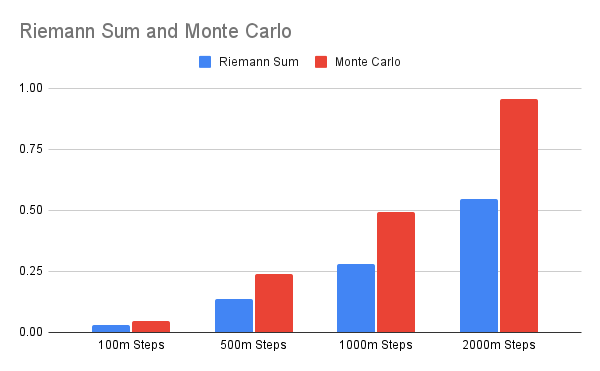
\includegraphics[width=\linewidth]{Images/riemann_monte_performance.png}
\captionof{figure}{Riemann Sum vs Monte Carlo Performance}
As we can see, the Riemann Sum is nearly twice as fast as the Monte Carlo. This is likely due to the computationally expensive process of generating a random number. Let us examine accuracy. The average difference between the Riemann Sum calculation and the Monte Carlo approximation between the actual value of $\pi$ are shown below. 
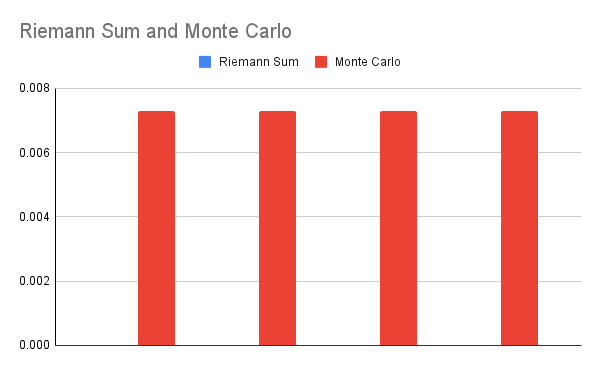
\includegraphics[width=\linewidth]{Images/riemann_monte.png}
\captionof{figure}{Riemann Sum vs Monte Carlo Accuracy}
As we can (not) see, the accuracy of the Riemann Sum method is so high that we cannot visually detect this in the graph. The Riemann sum accuracy was so high that at 100,000,000 steps, it had already approximated past the $10^{th}$ decimal place meaning all Riemann Sum calculations arrived at the same answer: 3.1415926736 at a difference of 0.00000002009999989 from $\pi$. This incredibly impressive algorithm will serve as the metric to analyze performance for the rest of the paper.

\section{Thread Counts and Step Size}
When running the processes, we varied the thread sizes on each iteration of step sizes, iterating over $7, 14, 21, 28$. Each thread created would execute on one CPU on the same node in Talapas. We created the SLURM script such that there was also 1 task per node and $n$ CPUs allocated when $n$ threads were created, with a maximum of 28 as there are only 28 available CPUs per node. We anticipate that an increase in thread count will provide a reduction in runtime. We know by Amdahl's Law that going from 1 to 28 CPUs will not result in a 28x speedup. However, we still expect to see a sizable speedup of around a magnitude greater. We vary the number of threads generated per process while keeping a constant of 100,000,000 steps. We will use atomic variables instead of critical sections here, but, as shown above, the difference between the two is insignificant. 
We will also vary the step size over $100,000,000$, $500,000,000$, $1,000,000,000$, $2,000,000,000$. $100,000,000$ serves as a baseline as we still observe relatively high accuracy while being significantly less computationally expensive. As we see, the relative difference in operations is 1x, 5x, 10x, 20x. This allows us to get a good reference to the tradeoffs between accuracy and performance.

The results are shown below. Results for the Monte Carlo method are not shown as the same pattern is observed.
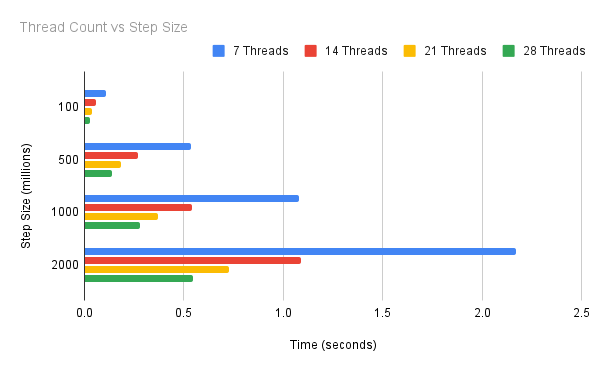
\includegraphics[width=\linewidth]{Images/chart.png}
\captionof{figure}{Atomic vs Critical : 100,000,000 steps with Varying Thread Count}
As we can see, the increase in performance is relatively logarithmic. This seems to obey Amdahl's Law as the increase in performance starts with being proportional to the increase in resources but begins to decline. We see that the jump from 7 CPUs allocated to 14 CPUs results in a 2x increase in performance across all numbers of steps, proportional to the 2x resources allocated. We see from then on the performance increase drops below 2x the previous at every new resource increase. By this, we can conclude that parallelism is very beneficial but suffers from the law of diminishing returns.

\section{Conclusion}
Due to the relatively simplistic nature of our project, our code was highly parallelizable. We observed dramatic speed-ups on both implementations of calculating $\pi$. This allows us to conclude that parallelism is extremely beneficial and allows us to observe performance that would be impossible to achieve without parallelism. We see that there is a constant rivalry between accuracy vs performance. This project highlights this and shows that effective performance and high accuracy can often be achieved through parallelism.


\end{multicols}

\end{document}
